\documentclass[11pt,a4paper]{article}

% ------------------------------------------------------------------
% Paquetes
% ------------------------------------------------------------------
\usepackage[utf8]{inputenc}
\usepackage[T1]{fontenc}
\usepackage[spanish,es-tabla,es-noshorthands]{babel}
\usepackage{lmodern}
\usepackage[margin=2.5cm]{geometry}
\usepackage{graphicx}
\usepackage{booktabs}
\usepackage{float}
\usepackage{caption}
\usepackage{subcaption}
\usepackage{amsmath}
\usepackage{enumitem}
\usepackage{tikz}
\usetikzlibrary{positioning,babel}
\usepackage[hidelinks]{hyperref}

\graphicspath{{figuras/}}
\setlist{itemsep=2pt}

% ------------------------------------------------------------------
% Datos del grupo (completar)
% ------------------------------------------------------------------
\newcommand{\grupo}{[Identificador del grupo]}
\newcommand{\repo}{https://github.com/VannaNotGianna/segmentacion-nube-puntos-3d}

\begin{document}

% ------------------------------------------------------------------
% Portada
% ------------------------------------------------------------------
\begin{titlepage}
  \centering
  {\large UTEC -- Universidad de Ingeniería y Tecnología\par}
  \vspace{0.5cm}
  {\large Machine Learning\par}
  \vspace{3cm}
  {\LARGE\bfseries Actividad 3\par}
  \vspace{0.4cm}
  {\Huge\bfseries Segmentación de una nube de puntos 3D mediante clustering\par}
  \vspace{3cm}
  {\large\textbf{Docente:} Jan Hurtado\par}
  \vspace{0.8cm}
  {\large\textbf{Grupo:} \grupo\par}
  \vspace{0.8cm}
  {\large\textbf{Integrantes}\par}
  \vspace{0.3cm}
  {\large
    Elizabeth Huamán Santillán\\
    Marialejandra [Apellidos]\\
    Joaquín [Apellidos]\par}
  \vfill
  {\large \today\par}
\end{titlepage}

% ------------------------------------------------------------------
\section{Introducción}
% ------------------------------------------------------------------
El objetivo de la actividad es segmentar los objetos presentes en una nube de
puntos 3D de una fábrica (pisos, techos, columnas, tuberías, vigas, entre
otros) utilizando algoritmos de clustering. La nube, capturada con un escáner
FARO, contiene \textbf{1\,647\,021 puntos}, cada uno con posición (XYZ), color
(RGB) y normal. El eje Z es vertical: el piso se encuentra a
$z \approx -1.7$\,m y el techo a $z \approx 8.7$\,m.

Se propone un procedimiento en varias etapas que combina \textbf{K-Means} y
\textbf{DBSCAN}, aprovechando en cada etapa el atributo más informativo:
primero la orientación de las normales, luego la posición y finalmente el
color.

% ------------------------------------------------------------------
\section{Procedimiento}
% ------------------------------------------------------------------

\subsection{Visión general}

La Figura~\ref{fig:pipeline} resume el procedimiento. La idea central es
separar primero los elementos estructurales grandes (piso, techo y columnas),
que conectan físicamente al resto de objetos, para que después DBSCAN pueda
separar los objetos restantes.

\begin{figure}[H]
  \centering
  \begin{tikzpicture}[
      node distance=4mm,
      etapa/.style={draw, rounded corners, align=center, text width=12.5cm,
                    inner sep=5pt, font=\small},
      flecha/.style={->, thick}]
    \node[etapa] (pre) {\textbf{Preprocesamiento:} submuestreo por vóxel (0.08\,m) y filtro de outliers};
    \node[etapa, below=of pre] (e1a) {\textbf{Etapa 1a -- Orientación:} K-Means ($k=3$) sobre $|\mathbf{n}|$};
    \node[etapa, below=of e1a] (e1b) {\textbf{Etapa 1b -- Superficies:} DBSCAN sobre XYZ de los puntos horizontales $\Rightarrow$ piso, techo, plataformas};
    \node[etapa, below=of e1b] (e2a) {\textbf{Etapa 2a -- Columnas:} cobertura vertical en planta + DBSCAN 2D sobre XY};
    \node[etapa, below=of e2a] (e2b) {\textbf{Etapa 2b -- Materiales:} K-Means ($k=5$) sobre el color};
    \node[etapa, below=of e2b] (e2c) {\textbf{Etapa 2c -- Objetos:} DBSCAN por material + reglas de material y altura $\Rightarrow$ tubería, viga/estructura, maquinaria};
    \node[etapa, below=of e2c] (e2e) {\textbf{Etapa 2d -- Suavizado:} voto mayoritario entre los 10 vecinos más cercanos};
    \node[etapa, below=of e2e] (tr) {\textbf{Transferencia:} cada punto de la nube original toma la clase del vecino más cercano};
    \foreach \a/\b in {pre/e1a, e1a/e1b, e1b/e2a, e2a/e2b, e2b/e2c, e2c/e2e, e2e/tr}
      \draw[flecha] (\a) -- (\b);
  \end{tikzpicture}
  \caption{Etapas del procedimiento de segmentación.}
  \label{fig:pipeline}
\end{figure}

\subsection{Preprocesamiento}

La nube se submuestrea con una grilla de vóxeles de 0.08\,m: los puntos de cada
vóxel se reemplazan por su promedio (posición, color y normal, renormalizada a
longitud 1). Luego se eliminan puntos aislados con un filtro estadístico
(20 vecinos, 2 desviaciones estándar). La nube queda con \textbf{454\,898
puntos}. El tamaño de 0.08\,m conserva perfiles y tuberías delgadas y permite
que DBSCAN se ejecute en segundos.

\subsection{Etapa 1: estructura (piso, techo y plataformas)}

\paragraph{1a. Orientación.} Se aplica K-Means con $k=3$ sobre el valor absoluto
de las normales $(|n_x|, |n_y|, |n_z|)$. Se usa el valor absoluto porque $\mathbf{n}$
y $-\mathbf{n}$ describen la misma superficie. Los tres clusters corresponden a
superficies horizontales y a superficies verticales orientadas según X y según
Y (centroides con componente dominante entre 0.91 y 0.97). El valor $k=3$ obtuvo
el mayor coeficiente de silhouette (0.695) y el menor índice de Davies-Bouldin
(0.526) entre $k=2$ y $k=6$.

\paragraph{1b. Superficies horizontales.} Agrupar los puntos horizontales solo
por altura no funciona, porque el piso tiene un desnivel de unos 10\,cm. En su
lugar se aplica DBSCAN ($\varepsilon = 0.15$\,m, 8 puntos mínimos) sobre la
posición XYZ, lo que separa superficies conexas. Cada superficie se etiqueta
según su altura y tamaño:
\begin{itemize}
  \item \textbf{Piso:} la superficie más baja entre las de mayor tamaño.
  \item \textbf{Techo:} superficies en los 1.5\,m superiores de la nube.
  \item \textbf{Plataforma:} superficies intermedias de más de 10\,m$^2$.
\end{itemize}

\begin{figure}[H]
  \centering
  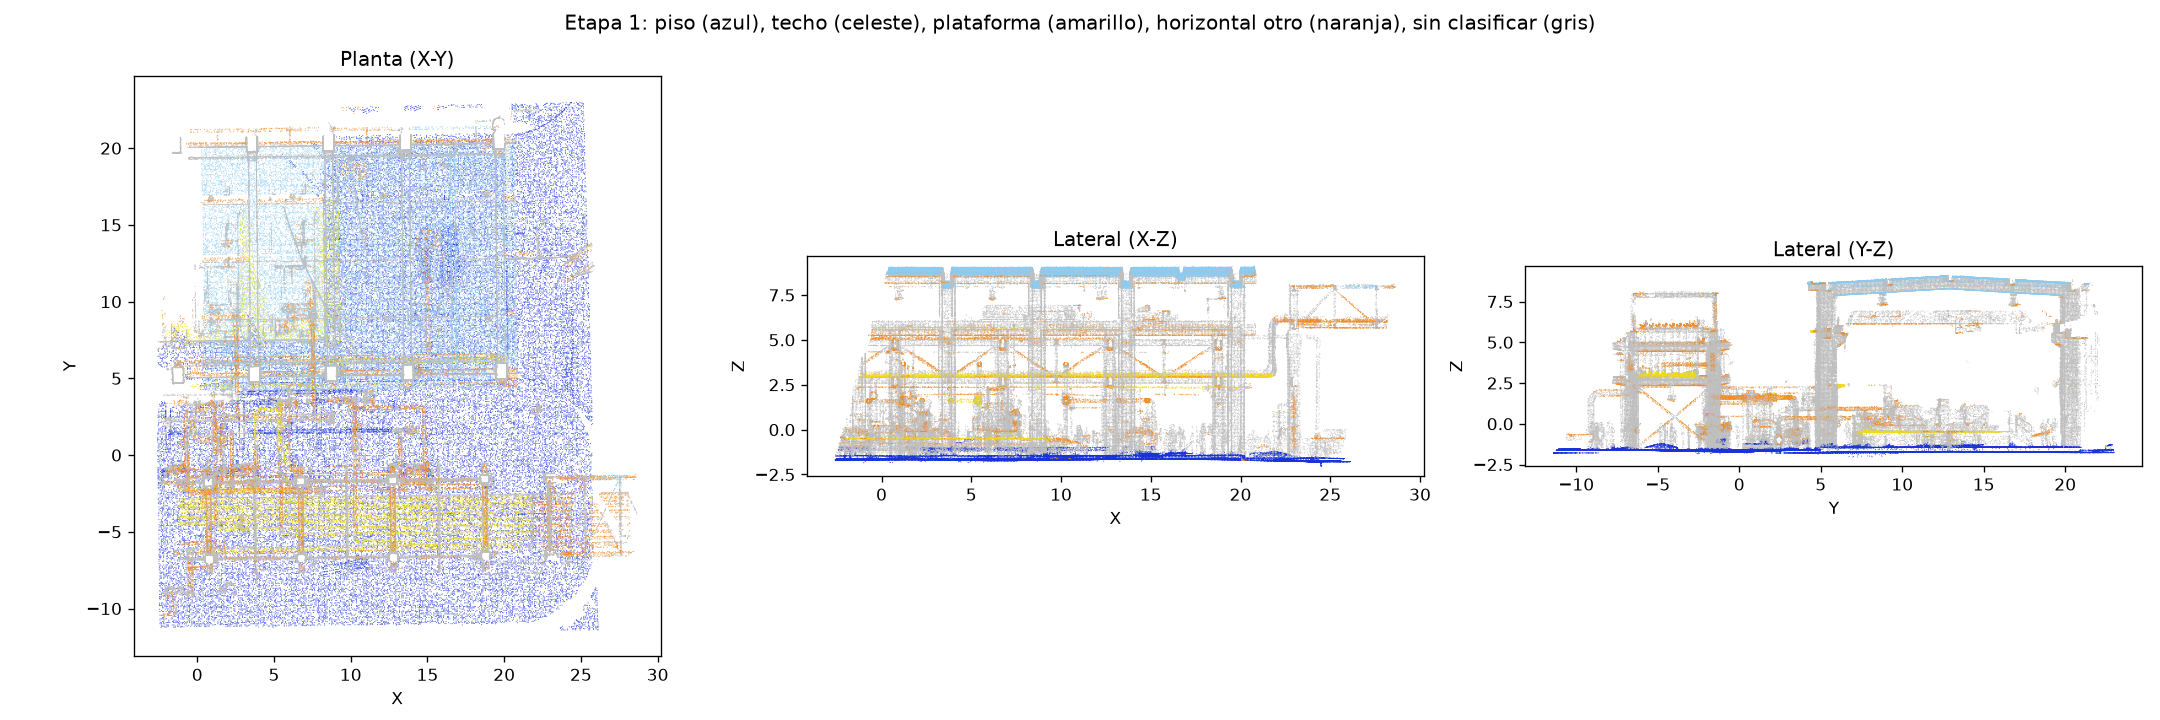
\includegraphics[width=\textwidth]{02_estructura.png}
  \caption{Resultado de la etapa 1 en planta y vistas laterales. Los puntos grises
    aún no están clasificados y pasan a la etapa 2.}
  \label{fig:etapa1}
\end{figure}

\subsection{Etapa 2: objetos}

Al aplicar DBSCAN directamente sobre los puntos restantes, columnas, vigas y
tuberías quedan unidas en un solo objeto que contiene el 91\,\% de los puntos.
Por eso los objetos se separan en varios pasos.

\paragraph{2a. Columnas.} La planta se divide en celdas de 0.25\,m y la altura
en franjas de 0.5\,m. Una columna ocupa casi toda la altura de su celda, por lo
que se seleccionan las celdas con al menos 5\,m de altura ocupada y se agrupan
con DBSCAN en 2D (solo XY). Se aceptan como columnas los grupos con una huella
menor a 2.5\,m por lado (Figura~\ref{fig:columnas}). Se detectaron 27 elementos
verticales: las columnas de ambas estructuras y algunos elementos verticales
delgados (de unos 20\,cm de ancho, probablemente tuberías verticales o postes).
Al retirarlos, el objeto más grande pasa del 91\,\% al 49\,\% de los puntos.

\begin{figure}[H]
  \centering
  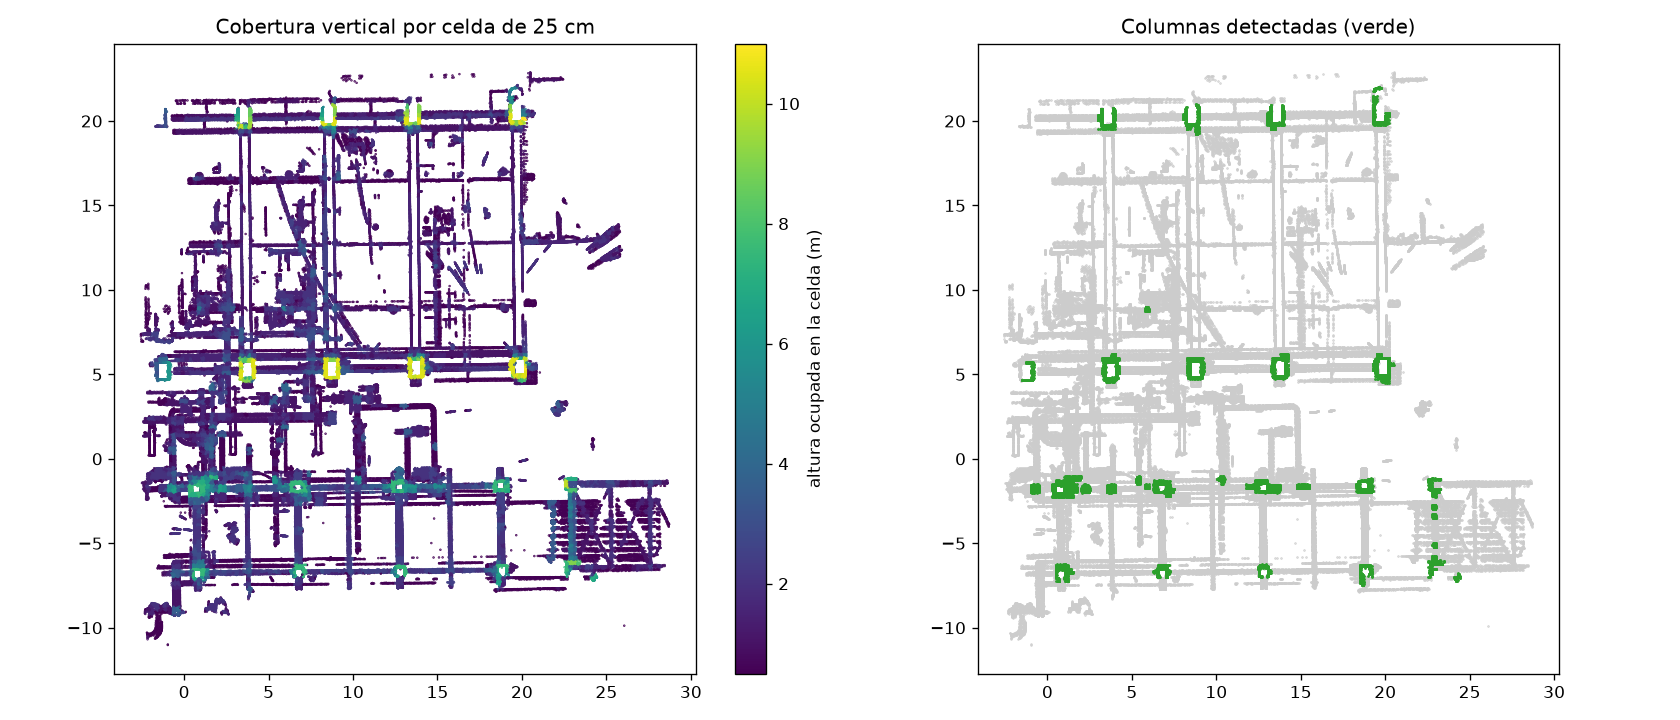
\includegraphics[width=\textwidth]{11_columnas.png}
  \caption{Izquierda: altura ocupada por celda. Derecha: columnas detectadas (verde).}
  \label{fig:columnas}
\end{figure}

\paragraph{2b. Materiales.} El componente que aún queda unido contiene una
estructura metálica verde, tuberías claras y máquinas oscuras, que se
distinguen por su color. Se aplica K-Means con $k=5$ sobre las características
de color $(s\cos 2\pi h,\; s\sin 2\pi h,\; v)$, donde $h$, $s$ y $v$ son el tono, la
saturación y el brillo. El tono se representa como un ángulo y se pondera por la
saturación para que los grises no tengan un tono arbitrario. Cada cluster se
asigna a un material según su color medio (Tabla~\ref{tab:materiales} y
Figura~\ref{fig:materiales}).

\begin{table}[H]
  \centering
  \begin{tabular}{lll}
    \toprule
    Color medio (RGB) & Material & Objetos típicos \\
    \midrule
    (0.69, 0.73, 0.75) & claro  & tuberías \\
    (0.39, 0.53, 0.32) & verde  & estructura metálica, arriostres \\
    (0.42, 0.23, 0.17) & óxido  & rieles del puente grúa \\
    (0.19, 0.18, 0.26) & oscuro & máquinas, puente grúa \\
    (0.29, 0.25, 0.25) & oscuro & cerchas del techo, máquinas \\
    \bottomrule
  \end{tabular}
  \caption{Clusters de color obtenidos con K-Means y material asignado.}
  \label{tab:materiales}
\end{table}

\begin{figure}[H]
  \centering
  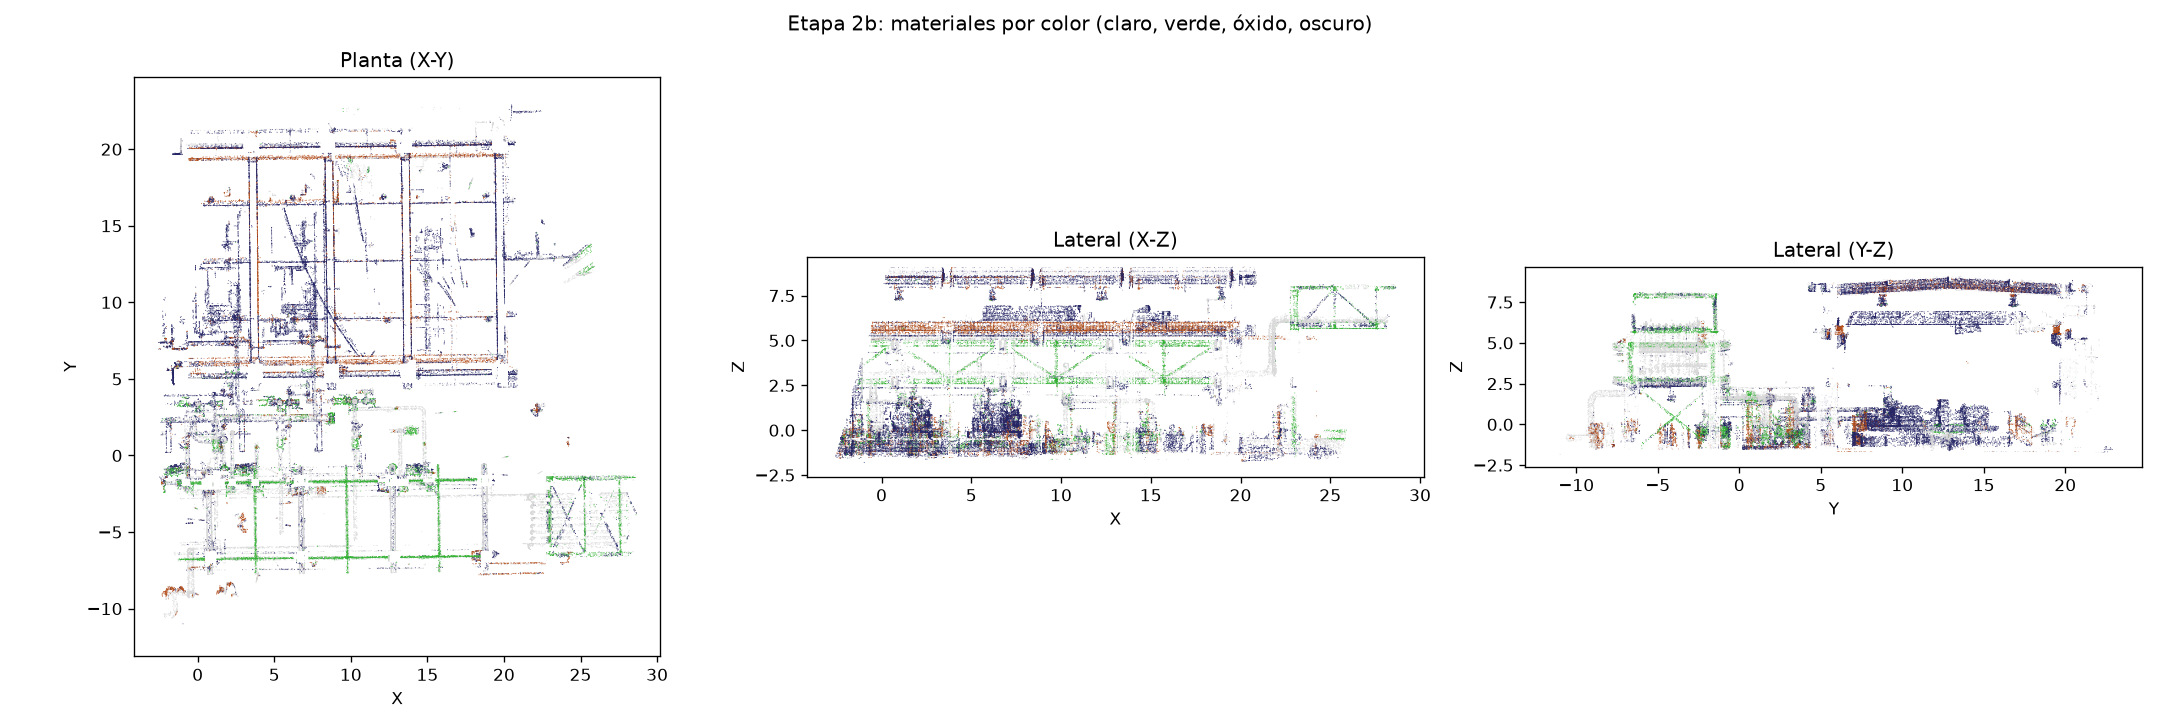
\includegraphics[width=\textwidth]{03_materiales_color.png}
  \caption{Materiales obtenidos con K-Means sobre el color.}
  \label{fig:materiales}
\end{figure}

\paragraph{2c. Objetos y clases.} Dentro de cada material se aplica DBSCAN
($\varepsilon = 0.2$\,m) para separar objetos individuales (1\,098 objetos). Cada
objeto recibe una clase según su material y su altura sobre el piso:
\begin{itemize}
  \item material claro $\Rightarrow$ \textbf{tubería};
  \item objeto elevado (base a más de 3\,m) o material verde $\Rightarrow$
        \textbf{viga / estructura metálica};
  \item material oscuro u óxido con mediana de altura menor a 2.5\,m
        $\Rightarrow$ \textbf{maquinaria};
  \item resto $\Rightarrow$ \textbf{otros}.
\end{itemize}
Los puntos que DBSCAN marca como ruido toman la clase del punto clasificado más
cercano.

\paragraph{2d. Suavizado.} Cada punto toma la clase mayoritaria entre sus 10
vecinos más cercanos, lo que corrige puntos aislados mal clasificados por
variaciones de color.

\subsection{Transferencia a la nube original}

Las clases se obtuvieron sobre la nube submuestreada. Para exportar la nube
completa, cada uno de los 1\,647\,021 puntos originales toma la clase del punto
submuestreado más cercano, que equivale a heredar la clase de su vóxel. El
99\,\% de los puntos está a menos de 5.3\,cm de su vecino. Los 8\,123 puntos a más
de 0.16\,m (los eliminados por el filtro de outliers) se asignan a la clase
\emph{otros}.

\subsection{Justificación de los métodos}

La elección de cada algoritmo sigue los criterios vistos en la sesión de
clustering del curso~\cite{curso}:

\begin{itemize}
  \item \textbf{K-Means para orientación y color.} En ambos casos se buscan
        grupos compactos en un espacio de pocas dimensiones. Como K-Means puede
        detenerse en un mínimo local según su inicialización, se usan varias
        inicializaciones (\texttt{n\_init}): 10 para la orientación y 30 para el
        color. Con 10 inicializaciones, el K-Means de color daba resultados
        distintos según la semilla aleatoria; con 30 todas las semillas
        coinciden en más del 99.8\,\% de los puntos.
  \item \textbf{$k$ es una decisión; el codo y la silhouette son indicios.}
        Para la orientación los indicios coinciden en $k=3$. Para el color, la
        silhouette se mantiene en torno a 0.35 para todo $k$ entre 2 y 8, sin un
        óptimo claro. Se eligió $k=5$ porque cada cluster corresponde a un
        material reconocible, y se verificó que los grupos tengan sentido para
        la tarea, ya que un clustering siempre devuelve los $k$ grupos pedidos.
  \item \textbf{DBSCAN para la separación espacial.} Los objetos tienen formas
        arbitrarias (tuberías curvas, estructuras en celosía) y hay puntos
        aislados que deben quedar como ruido, situaciones en las que K-Means
        falla y DBSCAN funciona bien. DBSCAN se aplica solo sobre la posición
        (pocas dimensiones), y el submuestreo por vóxel homogeneiza la
        densidad, ya que el escáner genera más puntos cerca de su posición y
        DBSCAN usa un único $\varepsilon$.
  \item \textbf{Un $\varepsilon$ estable.} Al cambiar el $\varepsilon$ de
        superficies de 0.15 a 0.20\,m, o el $\varepsilon$ de objetos entre 0.15
        y 0.25\,m, más del 98\,\% de los puntos conserva su clase. En cambio, con
        un $\varepsilon$ de superficies de 0.10\,m, valor cercano a la
        separación entre puntos, el 71\,\% de los puntos horizontales queda como
        ruido y el piso deja de reconocerse.
  \item \textbf{Unidades.} Ninguna etapa combina atributos con unidades
        distintas: las normales están entre 0 y 1, la posición en metros y las
        características de color son adimensionales. Por eso no fue necesario
        estandarizar, y cada atributo se usa en la etapa donde es más
        informativo en lugar de mezclarlos en una sola distancia.
  \item \textbf{Métodos no utilizados.} El clustering jerárquico requiere
        todas las distancias entre pares de puntos: con 454\,898 puntos son unos
        $10^{11}$ pares (cerca de 800\,GB de memoria), por lo que no es viable.
        Un modelo de mezcla gaussiana sería una alternativa para la etapa de
        color, donde los grupos se superponen, y podría indicar qué tan segura
        es la asignación de cada punto.
\end{itemize}

% ------------------------------------------------------------------
\section{Resultados}
% ------------------------------------------------------------------

La Tabla~\ref{tab:conteo} muestra la distribución de clases en la nube original
y las Figuras~\ref{fig:vistas} y~\ref{fig:proyecciones} muestran la nube
segmentada. Las capturas se generaron con Open3D; la nube exportada puede
abrirse también en CloudCompare o MeshLab.

\begin{table}[H]
  \centering
  \begin{tabular}{llrr}
    \toprule
    Clase & Color & Puntos & \% \\
    \midrule
    Piso                       & azul     & 493\,411 & 30.0 \\
    Columna                    & verde    & 283\,708 & 17.2 \\
    Viga / estructura metálica & morado   & 258\,708 & 15.7 \\
    Techo                      & celeste  & 208\,994 & 12.7 \\
    Tubería                    & rojo     & 161\,992 &  9.8 \\
    Maquinaria                 & naranja  & 140\,026 &  8.5 \\
    Plataforma                 & amarillo &  87\,446 &  5.3 \\
    Otros                      & gris     &  12\,736 &  0.8 \\
    \midrule
    Total                      &          & 1\,647\,021 & 100.0 \\
    \bottomrule
  \end{tabular}
  \caption{Puntos por clase en la nube original segmentada.}
  \label{tab:conteo}
\end{table}

\begin{figure}[H]
  \centering
  \begin{subfigure}{0.49\textwidth}
    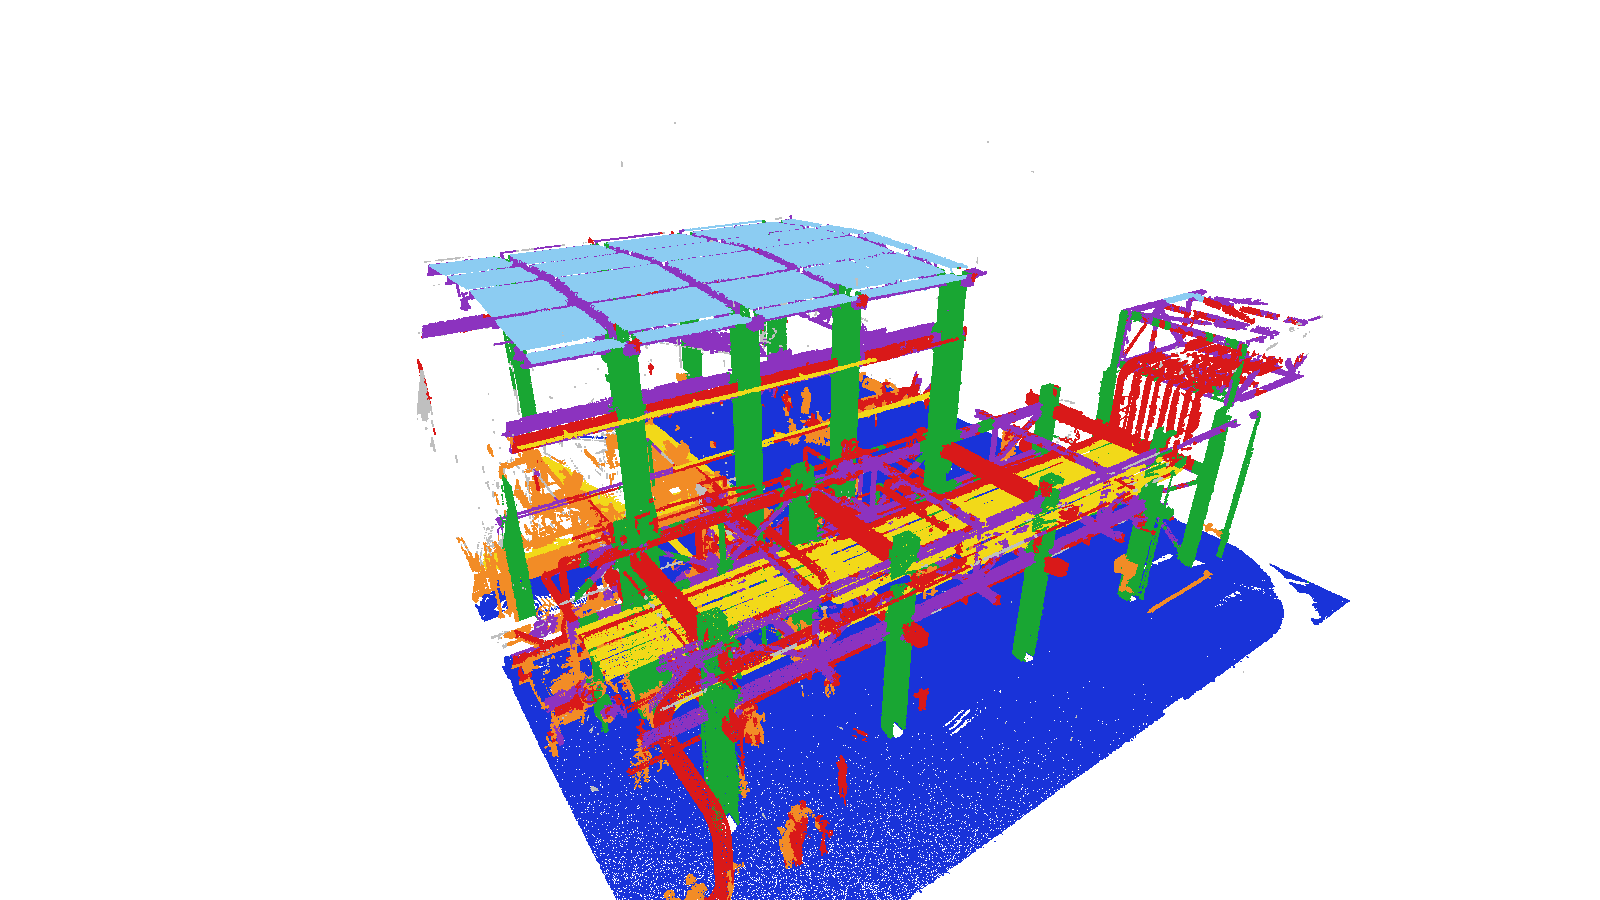
\includegraphics[width=\textwidth]{20_vista_aerea.png}
    \caption{Vista aérea.}
  \end{subfigure}\hfill
  \begin{subfigure}{0.49\textwidth}
    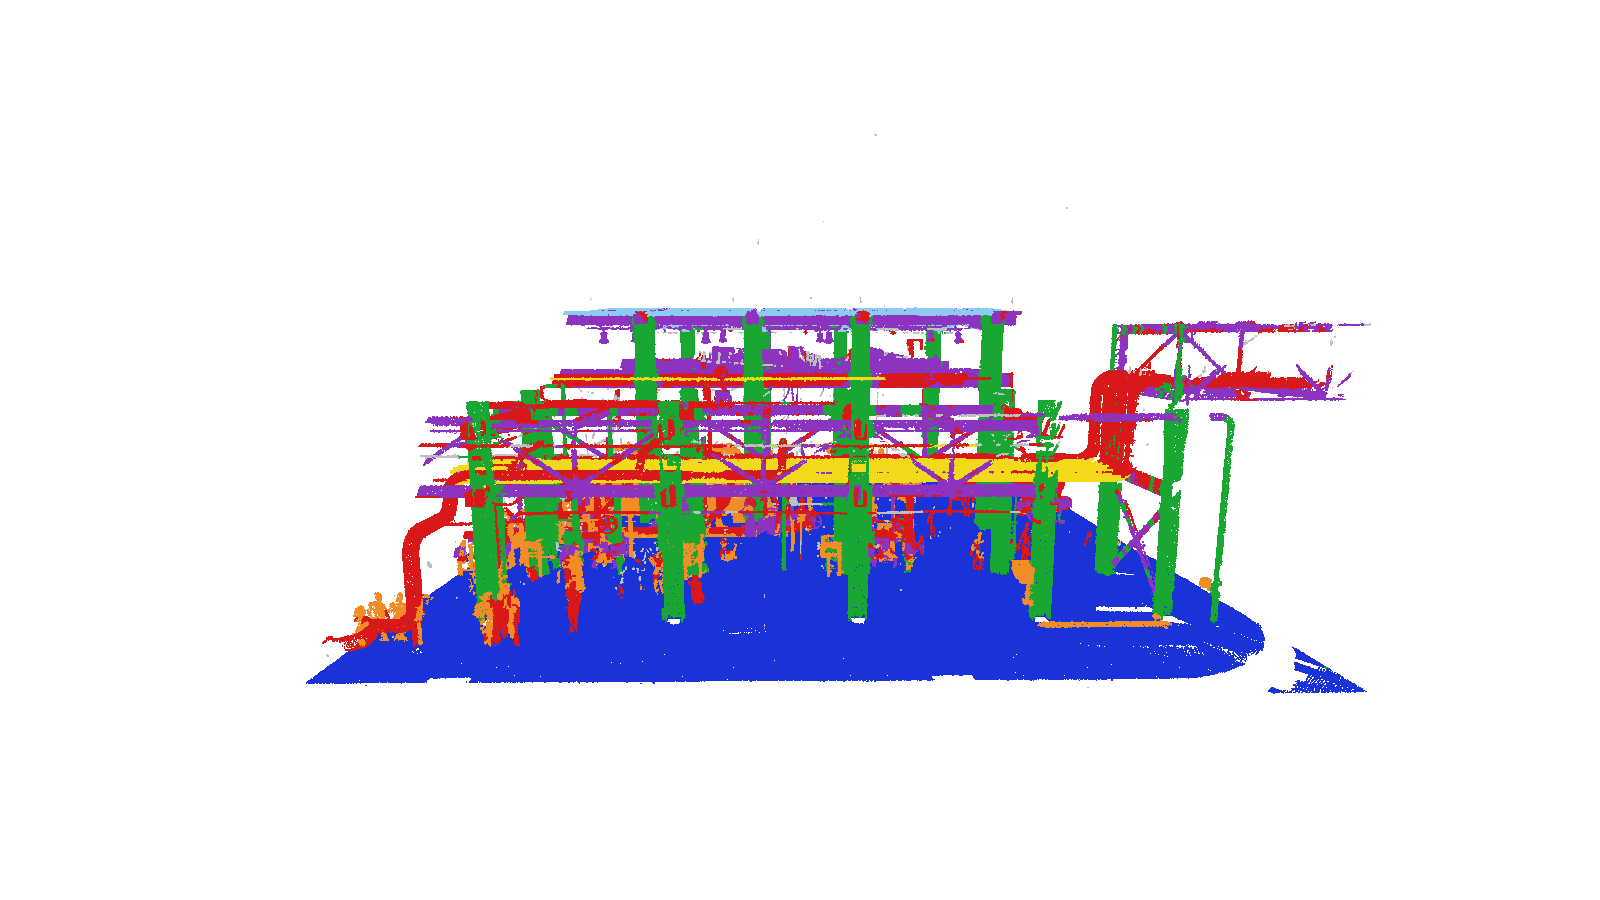
\includegraphics[width=\textwidth]{20_vista_lateral.png}
    \caption{Vista lateral.}
  \end{subfigure}

  \vspace{2mm}
  \begin{subfigure}{0.49\textwidth}
    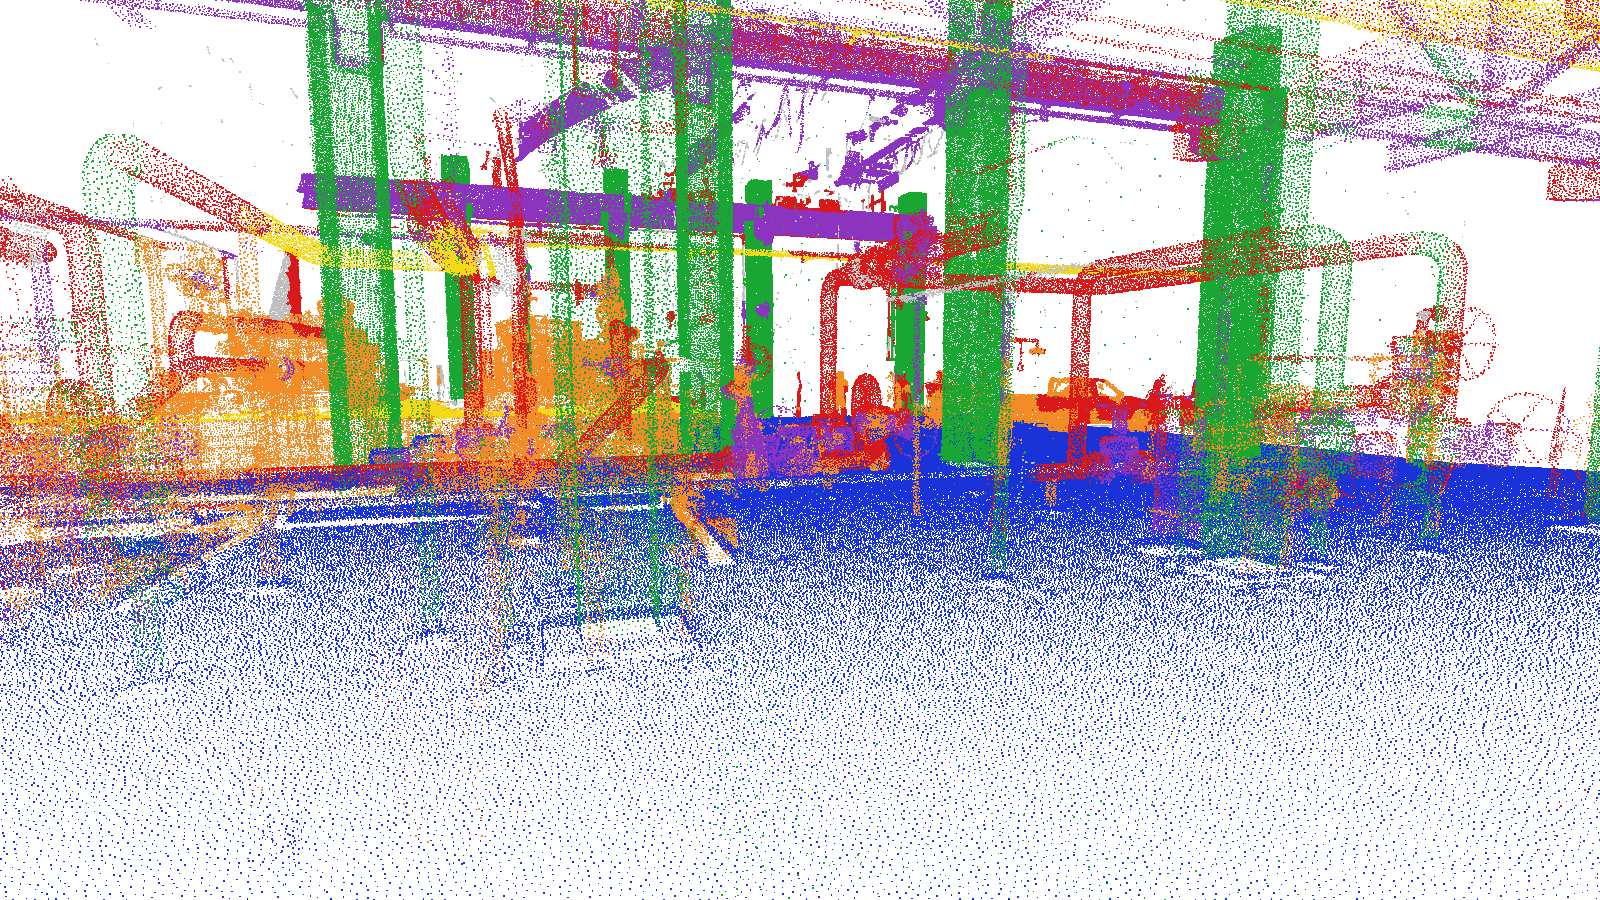
\includegraphics[width=\textwidth]{20_vista_interior_nave.png}
    \caption{Interior de la nave (sin techo).}
  \end{subfigure}\hfill
  \begin{subfigure}{0.49\textwidth}
    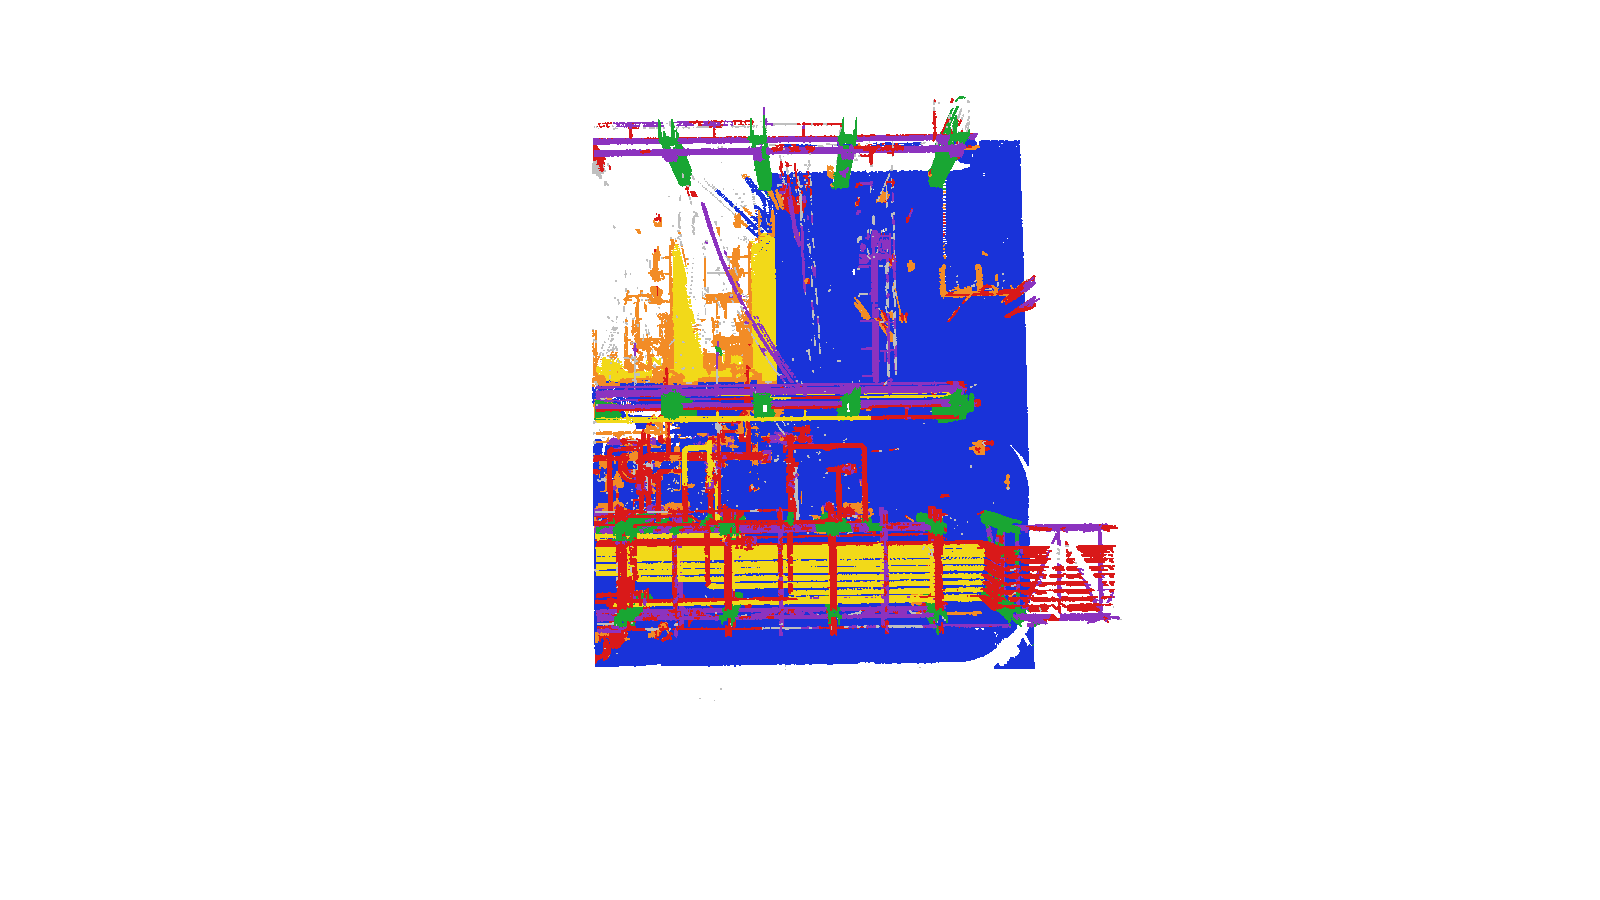
\includegraphics[width=\textwidth]{20_vista_planta.png}
    \caption{Planta (sin techo).}
  \end{subfigure}

  \vspace{2mm}
  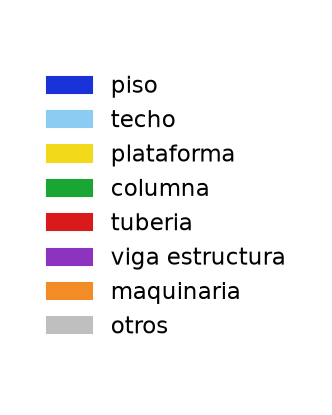
\includegraphics[width=0.22\textwidth]{21_leyenda.png}
  \caption{Nube de puntos segmentada (nube original completa).}
  \label{fig:vistas}
\end{figure}

\begin{figure}[H]
  \centering
  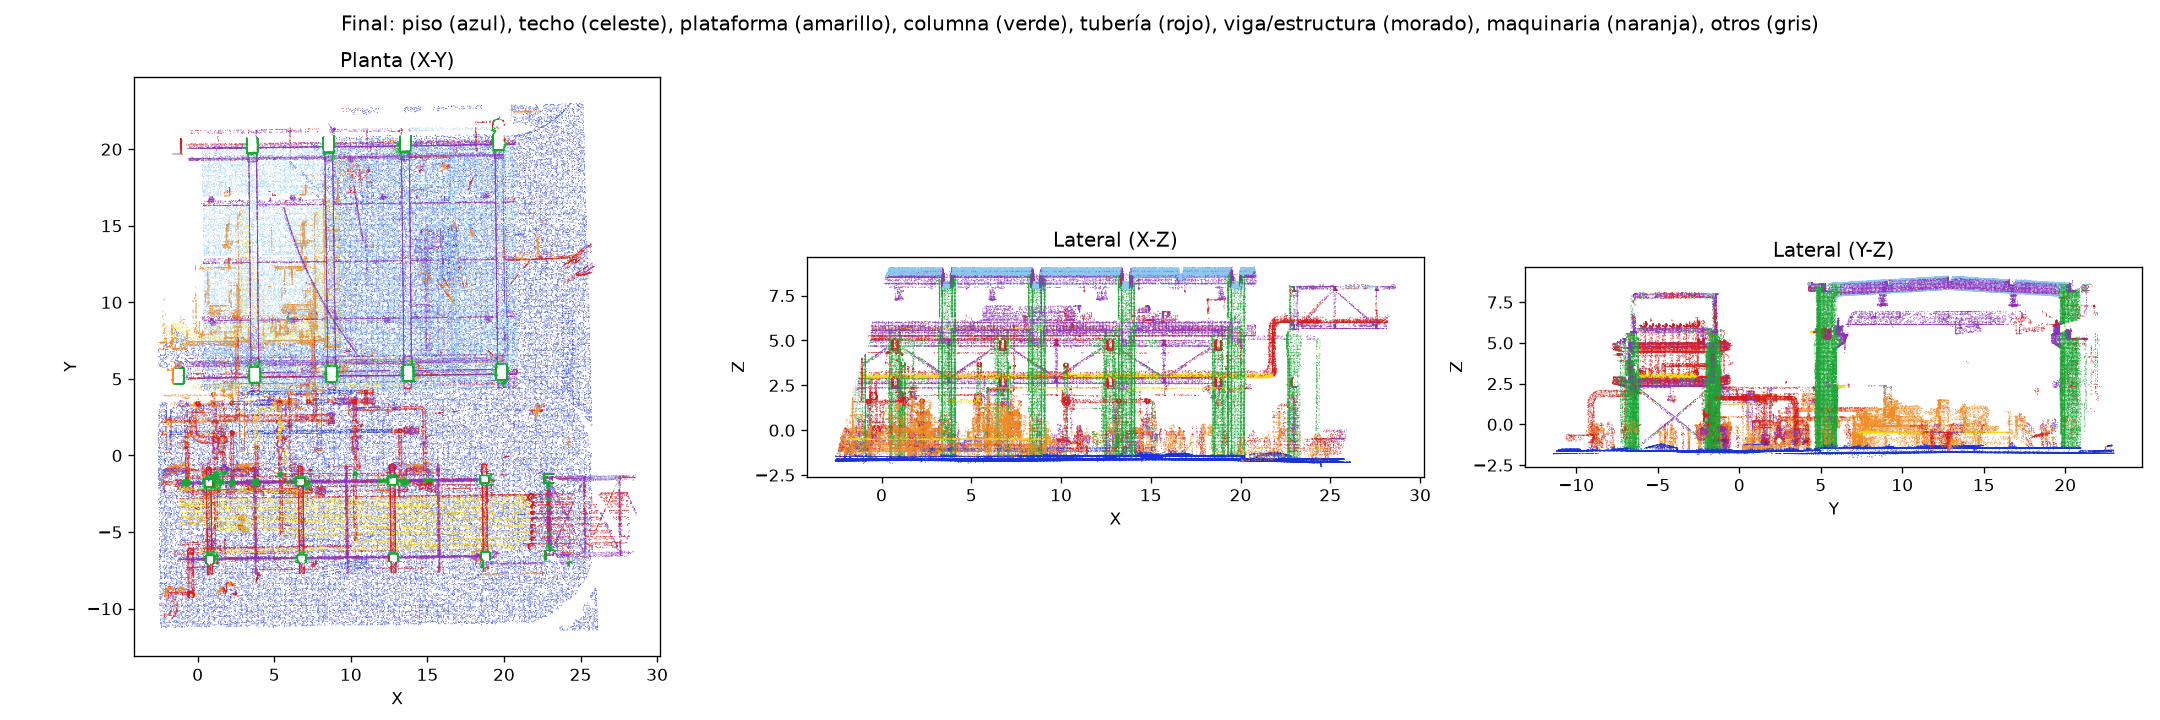
\includegraphics[width=\textwidth]{05_segmentacion_final.png}
  \caption{Segmentación final en planta y vistas laterales.}
  \label{fig:proyecciones}
\end{figure}

Se identifican correctamente el piso, los paneles del techo, las plataformas,
las columnas de ambas estructuras, la red de tuberías, las vigas, los rieles del
puente grúa y la estructura metálica, así como la maquinaria apoyada en el piso.

\paragraph{Limitaciones.}
\begin{itemize}
  \item No se detectaron personas ni vehículos como clases propias: no se
        encontraron ejemplos claros en la nube y su forma se confunde con la
        maquinaria.
  \item Las reglas de clasificación dependen de esta escena (por ejemplo,
        ``material claro = tubería'').
  \item Los colores no forman grupos bien separados (silhouette $\approx 0.35$),
        por lo que la etapa de color es la más sensible a los parámetros.
\end{itemize}

% ------------------------------------------------------------------
\section{Código y archivos entregados}
% ------------------------------------------------------------------
\begin{itemize}
  \item \textbf{Código fuente:} \url{\repo}. Las instrucciones de instalación y
        ejecución están en el archivo \texttt{README.md}. La segmentación
        completa se ejecuta con \texttt{python -m src.pipeline}.
  \item \textbf{Nube segmentada:} \texttt{segmentacion\_final\_completa.ply}
        (nube original completa con un color por clase).
\end{itemize}

% ------------------------------------------------------------------
\begin{thebibliography}{9}
% ------------------------------------------------------------------
\bibitem{curso} J. Hurtado. Lecture 10 -- Clustering: the intuitive version.
  Curso de Machine Learning, UTEC, 2026.
\bibitem{dbscan} M. Ester, H.-P. Kriegel, J. Sander y X. Xu. A density-based
  algorithm for discovering clusters in large spatial databases with noise.
  \emph{Proceedings of KDD}, 1996.
\bibitem{kmeans} S. Lloyd. Least squares quantization in PCM.
  \emph{IEEE Transactions on Information Theory}, 28(2):129--137, 1982.
\bibitem{sklearn} F. Pedregosa et al. Scikit-learn: Machine Learning in Python.
  \emph{Journal of Machine Learning Research}, 12:2825--2830, 2011.
\bibitem{open3d} Q.-Y. Zhou, J. Park y V. Koltun. Open3D: A modern library for
  3D data processing. \emph{arXiv:1801.09847}, 2018.
\end{thebibliography}

\end{document}
